\clearpage
\section{Model inspection: 1-lepton channel}
\label{sec:fit_1lep}

We show the results for the model inspection and discuss the goodness of the fit model for the \olep channel
in this section.

\subsection{Prefit plots}

%%%Figure \ref{fig:fit_1lep_prefit} shows the pre-fit plots of the analysis regions entering in the \olep fit only model; 
%%%in particular, \mjjtag distributions in \Wjets and top CRs are shown and the neural network scores distributions 
%%%are shown in the SRs, only the left side bins are plotted using real data as well.

Figure \ref{fig:fit_1lep_prefit} presents the pre-fit plots for the analysis regions included in the one-lepton fit model. 
It features the distributions of DNN scores in the SRs, as well as the \mjjtag distributions in the \Wjets and top CRs. 
Initially, only the bins on the left side were displayed with real data in the SRs, which have now been unblinded.

\begin{figure}[ht]
    \centering
    \begin{subfigure}[b]{0.32\textwidth}
        \includegraphics[width=\textwidth]{figures/FitResults/prefit/Region_distDNN_DSRVBSHP_BMin0_J0_incJet1_L1_T0_incFat1_Y6051_incTag1_Fat1_Prefitlog.pdf}
        \caption{Merged HP SR}
    \end{subfigure}
    \begin{subfigure}[b]{0.32\textwidth}
        \includegraphics[width=\textwidth]{figures/FitResults/prefit/Region_distDNN_DSRVBSLP_BMin0_J0_incJet1_L1_T0_incFat1_Y6051_incTag1_Fat1_Prefitlog.pdf}
        \caption{Merged LP SR}
    \end{subfigure}
    \begin{subfigure}[b]{0.32\textwidth}
        \includegraphics[width=\textwidth]{figures/FitResults/prefit/Region_distDNN_DSRVBSTight_BMin0_T0_Y6051_incTag1_J2_L1_incJet1_Prefitlog.pdf}
        \caption{Resolved SR}
    \end{subfigure}
    \\
    \begin{subfigure}[b]{0.32\textwidth}
        \includegraphics[width=\textwidth]{figures/FitResults/prefit/Region_disttagMjj_DCRVjetMerged_BMin0_J0_incJet1_L1_T0_incFat1_Y6051_incTag1_Fat1_Prefitlog.pdf}
        \caption{Merged WCR}
    \end{subfigure}
    \begin{subfigure}[b]{0.32\textwidth}
        \includegraphics[width=\textwidth]{figures/FitResults/prefit/Region_disttagMjj_DCRVjetTight_BMin0_T0_Y6051_incTag1_J2_L1_incJet1_Prefitlog.pdf}
        \caption{Resolved WCR}
    \end{subfigure}
    \\
    \begin{subfigure}[b]{0.32\textwidth}
        \includegraphics[width=\textwidth]{figures/FitResults/prefit/Region_disttagMjj_DCRTopHP_BMin0_J0_incJet1_L1_T0_incFat1_Y6051_incTag1_Fat1_Prefit.pdf}
        \caption{Merged HP TopCR}
    \end{subfigure}
    \begin{subfigure}[b]{0.32\textwidth}
        \includegraphics[width=\textwidth]{figures/FitResults/prefit/Region_disttagMjj_DCRTopLP_BMin0_J0_incJet1_L1_T0_incFat1_Y6051_incTag1_Fat1_Prefit.pdf}
        \caption{Merged LP TopCR}
    \end{subfigure}
    \begin{subfigure}[b]{0.32\textwidth}
        \includegraphics[width=\textwidth]{figures/FitResults/prefit/Region_disttagMjj_DCRTopTight_BMin0_T0_Y6051_incTag1_J2_L1_incJet1_Prefitlog.pdf}
        \caption{Resolved TopCR}
    \end{subfigure}
    \caption{Prefit plots for the 1 lepton channel. Data has been unblinded}
    \label{fig:fit_1lep_prefit}
\end{figure}

\clearpage
\subsection{Prefit tables}

Tables \ref{tab:1lepPrefitYield_SR}-\ref{tab:1lepPrefitYield_CR} shows the expected yields for signal and background processes 
in all the control and signal regions for the \olep channel.

%%\begin{table}
\centering
%\scalebox{0.85}{
\begin{tabular}{|l|c|}
\hline
\multicolumn{2}{|c|}{SRVBSHP L1}\\ \hline
W & 4238.22 $\pm$ 507.32\\
Z & 155.27 $\pm$ 28.21\\
Diboson & 584.89 $\pm$ 196.85\\
stop & 720.09 $\pm$ 248.44\\
ttbar & 7724.82 $\pm$ 1513.25\\
\hline
Bkg & 13423.28 $\pm$ 1920.49\\
\hline
EW6lvqq & 234.60 $\pm$ 42.30\\
\hline
Signal & 234.60 $\pm$ 42.30\\
SignalExpected & 234.60 $\pm$ 42.30\\
\hline
S/B & 1.75e-02\\
S/sqrt(S+B) & 2.01e+00\\ 
\hline
\end{tabular}
%}
%\end{table}
%\begin{table}
%\centering
%\small
%\scalebox{0.85}{
\begin{tabular}{|l|c|}
\hline
\multicolumn{2}{|c|}{SRVBSLP L1}\\ \hline
W & 12198.77 $\pm$ 1034.41\\
Z & 431.67 $\pm$ 69.13\\
Diboson & 788.97 $\pm$ 260.84\\
stop & 974.63 $\pm$ 312.95\\
ttbar & 10758.08 $\pm$ 1212.22\\
\hline
Bkg & 25152.11 $\pm$ 2238.93\\
\hline
EW6lvqq & 186.08 $\pm$ 37.97\\
\hline
Signal & 186.08 $\pm$ 37.97\\
SignalExpected & 186.08 $\pm$ 37.97\\
\hline
S/B & 7.40e-03\\
S/sqrt(S+B) & 1.17e+00\\
\hline
\end{tabular}
%}
%\end{table}
%\begin{table}
%\centering
%\small
%\scalebox{0.85}{
\begin{tabular}{|l|c|}
\hline
\multicolumn{2}{|c|}{SRVBSRes L1}\\ \hline
W & 60551.72 $\pm$ 5340.84\\
Z & 2090.52 $\pm$ 411.36\\
Diboson & 1781.12 $\pm$ 543.54\\
stop & 1750.76 $\pm$ 538.59\\
ttbar & 7330.60 $\pm$ 238.30\\
\hline
Bkg & 73504.70 $\pm$ 5960.54\\
\hline
EW6lvqq & 673.79 $\pm$ 56.53\\
\hline
Signal & 673.79 $\pm$ 56.53\\
SignalExpected & 673.79 $\pm$ 56.53\\
\hline
S/B & 9.17e-03\\
S/sqrt(S+B) & 2.47e+00\\
\hline
\end{tabular}
\caption{Prefit event yields for the analysis SRs in the 1 lepton channel.}
\label{tab:1lepPrefitYield_SR}
\end{table}


%%% second table
\begin{table}
\centering
%}
%\end{table}
%\begin{table}
%\centering
%\small
%\scalebox{0.85}{
\begin{tabular}{|l|c|}
\hline
\multicolumn{2}{|c|}{CRTopHP L1}\\ \hline
W & 328.01 $\pm$ 39.35\\
Z & 16.13 $\pm$ 2.80\\
Diboson & 43.58 $\pm$ 14.12\\
stop & 1342.33 $\pm$ 455.72\\
ttbar & 12266.87 $\pm$ 2348.67\\
\hline
Bkg & 13996.92 $\pm$ 2605.58\\
\hline
EW6lvqq & 82.34 $\pm$ 14.94\\
\hline
Signal & 82.34 $\pm$ 14.94\\
SignalExpected & 82.34 $\pm$ 14.94\\
\hline
S/B & 5.88e-03\\
S/sqrt(S+B) & 6.94e-01\\
\hline
data & 12195\\ \hline
\end{tabular}
%}
%\end{table}
%\begin{table}
%\centering
%\small
%\scalebox{0.85}{
\begin{tabular}{|l|c|}
\hline
\multicolumn{2}{|c|}{CRTopLP L1}\\ \hline
W & 869.04 $\pm$ 62.56\\
Z & 42.60 $\pm$ 6.00\\
Diboson & 67.82 $\pm$ 21.71\\
stop & 1426.00 $\pm$ 465.43\\
ttbar & 16507.86 $\pm$ 1911.45\\
\hline
Bkg & 18913.31 $\pm$ 2165.24\\
\hline
EW6lvqq & 67.74 $\pm$ 11.21\\
\hline
Signal & 67.74 $\pm$ 11.21\\
SignalExpected & 67.74 $\pm$ 11.21\\
\hline
S/B & 3.58e-03\\
S/sqrt(S+B) & 4.92e-01\\
\hline
data & 17195\\ \hline
\end{tabular}
%}
%\end{table}
%\clearpage
%\begin{table}
%\centering
%\small
%\scalebox{0.85}{
\begin{tabular}{|l|c|}
\hline
\multicolumn{2}{|c|}{CRTopRes L1}\\ \hline
W & 2092.06 $\pm$ 99.97\\
Z & 95.91 $\pm$ 13.64\\
Diboson & 87.60 $\pm$ 26.54\\
stop & 2132.56 $\pm$ 645.92\\
ttbar & 11362.88 $\pm$ 189.40\\
\hline
Bkg & 15771.01 $\pm$ 715.35\\
\hline
EW6lvqq & 155.16 $\pm$ 6.81\\
\hline
Signal & 155.16 $\pm$ 6.81\\
SignalExpected & 155.16 $\pm$ 6.81\\
\hline
S/B & 9.84e-03\\
S/sqrt(S+B) & 1.23e+00\\
\hline
data & 16131\\ \hline
\end{tabular} 
%}
%\end{table}
%\begin{table}
%\centering
%\small
%\scalebox{0.85}{
\begin{tabular}{|l|c|}
\hline
\multicolumn{2}{|c|}{CRVjetMer L1}\\ \hline

W & 39090.06 $\pm$ 3569.60\\
Z & 1326.81 $\pm$ 203.25\\
Diboson & 1702.72 $\pm$ 527.24\\
stop & 2523.47 $\pm$ 782.38\\
ttbar & 30085.03 $\pm$ 2277.28\\
\hline
Bkg & 74728.10 $\pm$ 5746.54\\
\hline
EW6lvqq & 175.02 $\pm$ 16.54\\
\hline
Signal & 175.02 $\pm$ 16.54\\
SignalExpected & 175.02 $\pm$ 16.54\\
\hline
S/B & 2.34e-03\\
S/sqrt(S+B) & 6.39e-01\\
\hline
data & 64166\\ \hline
\end{tabular}
%}
%\end{table}
%\begin{table}
%\centering
%\small
%\scalebox{0.85}{
\begin{tabular}{|l|c|}
\hline
\multicolumn{2}{|c|}{CRVjetRes L1}\\ \hline
W & 519953.24 $\pm$ 74295.68\\
Z & 20255.39 $\pm$ 5655.70\\
Diboson & 15746.59 $\pm$ 4922.41\\
stop & 33439.42 $\pm$ 10624.43\\
ttbar & 220957.70 $\pm$ 16705.73\\
\hline
Bkg & 810352.34 $\pm$ 100241.75\\
\hline
EW6lvqq & 1863.07 $\pm$ 149.73\\
\hline
Signal & 1863.07 $\pm$ 149.73\\
SignalExpected & 1863.07 $\pm$ 149.73\\
\hline
S/B & 2.30e-03\\
S/sqrt(S+B) & 2.07e+00\\
\hline
data & 788869\\ \hline
\end{tabular}
%}
\caption{Prefit event yields for the analysis CRs in the 1 lepton channel.}
\label{tab:1lepPrefitYield_CR}
\end{table}
%%% Local Variables:
%%% mode: latex
%%% TeX-master: "../../../../ANA-STDM-2018-27-INT1"
%%% End:
~


% \newcolumntype{d}{D{+}{\hspace{-3pt}\;\pm\;}{-1}}
%%%\documentclass{article}
%%%\usepackage{graphicx}
%%%\newcommand{\GeV}{\mathrm{GeV}}
%%%\newcommand{\ptv}{p_T^V}
%%%\begin{document}
\begin{table}[ht]
\centering
\small
\begin{tabular}{|l|c|}
\hline
\multicolumn{2}{|c|}{DNN\_SRVBSHP} \\ \hline
W & 4656.33 $\pm$ 599.26\\
Z & 155.86 $\pm$ 29.63\\
Diboson & 564.00 $\pm$ 208.79\\
stop & 720.09 $\pm$ 249.77\\
ttbar & 7724.82 $\pm$ 1531.65\\
\hline
Bkg & 13821.09 $\pm$ 2012.72\\
\hline
EW6lvqq & 228.59 $\pm$ 41.37\\
\hline
Signal & 228.59 $\pm$ 41.37\\
SignalExpected & 228.59 $\pm$ 41.37\\
\hline
S/B & 1.65e-02\\
S/sqrt(S+B) & 1.93e+00\\
\hline
data & 12178\\ \hline
\end{tabular}
%%%\end{table}
%%%
%%%
%%%\begin{table}
%%%\centering
%%%\small
\begin{tabular}{|l|c|}
\hline
 \multicolumn{2}{|c|}{DNN\_SRVBSLP}\\ \hline
W & 13507.48 $\pm$ 1306.67\\
Z & 433.51 $\pm$ 75.10\\
Diboson & 759.72 $\pm$ 276.17\\
stop & 974.63 $\pm$ 316.11\\
ttbar & 10758.23 $\pm$ 1251.68\\
\hline
Bkg & 26433.56 $\pm$ 2560.55\\
\hline
EW6lvqq & 180.21 $\pm$ 37.21\\
\hline
Signal & 180.21 $\pm$ 37.21\\
SignalExpected & 180.21 $\pm$ 37.21\\
\hline
S/B & 6.82e-03\\
S/sqrt(S+B) & 1.10e+00\\
\hline
data & 22158\\ \hline
\end{tabular}
%%%\end{table}
%%%
%%%
%%%\begin{table}
%%%\centering
%%%\small
\begin{tabular}{|l|c|}
\hline
 \multicolumn{2}{|c|}{DNN\_SRVBSRes}\\ \hline
W & 60551.72 $\pm$ 5916.55\\
Z & 2114.42 $\pm$ 425.26\\
Diboson & 1723.35 $\pm$ 582.92\\
stop & 1750.76 $\pm$ 541.16\\
ttbar & 7330.60 $\pm$ 299.18\\
\hline
Bkg & 73470.84 $\pm$ 6611.96\\
\hline
EW6lvqq & 662.01 $\pm$ 56.52\\
\hline
Signal & 662.01 $\pm$ 56.52\\
SignalExpected & 662.01 $\pm$ 56.52\\
\hline
S/B & 9.01e-03\\
S/sqrt(S+B) & 2.43e+00\\
\hline
data & 71272\\ \hline
\end{tabular}
\caption{Prefit event yields for the analysis SRs in the 1 lepton channel.}
\label{tab:1lepPrefitYield_SR}
\end{table}


\begin{table}
\centering
\small
\begin{tabular}{|l|c|}
\hline
 \multicolumn{2}{|c|}{tagMjj\_CRTopHP}\\ \hline
W & 352.82 $\pm$ 43.34\\
Z & 16.22 $\pm$ 3.13\\
Diboson & 41.79 $\pm$ 15.53\\
stop & 1342.33 $\pm$ 456.84\\
ttbar & 12267.00 $\pm$ 2374.62\\
\hline
Bkg & 14020.16 $\pm$ 2635.77\\
\hline
EW6lvqq & 72.15 $\pm$ 13.03\\
\hline
Signal & 72.15 $\pm$ 13.03\\
SignalExpected & 72.15 $\pm$ 13.03\\
\hline
S/B & 5.15e-03\\
S/sqrt(S+B) & 6.08e-01\\
\hline
data & 12195\\ \hline
\end{tabular}
%%%\end{table}
%%%
%%%
%%%\begin{table}
%%%\centering
%%%\small
\begin{tabular}{|l|c|}
\hline
 \multicolumn{2}{|c|}{tagMjj\_CRTopLP}\\ \hline
W & 949.62 $\pm$ 77.62\\
Z & 43.10 $\pm$ 7.66\\
Diboson & 65.63 $\pm$ 22.52\\
stop & 1426.00 $\pm$ 466.82\\
ttbar & 16508.02 $\pm$ 1970.36\\
\hline
Bkg & 18992.37 $\pm$ 2239.62\\
\hline
EW6lvqq & 59.17 $\pm$ 9.99\\
\hline
Signal & 59.17 $\pm$ 9.99\\
SignalExpected & 59.17 $\pm$ 9.99\\
\hline
S/B & 3.12e-03\\
S/sqrt(S+B) & 4.29e-01\\
\hline
data & 17195\\ \hline
\end{tabular}
%%%\end{table}
%%%
%%%
%%%\clearpage
%%%
%%%
%%%\begin{table}
%%%\centering
%%%\small
\begin{tabular}{|l|c|}
\hline
 \multicolumn{2}{|c|}{tagMjj\_CRTopRes}\\ \hline
W & 2092.27 $\pm$ 102.60\\
Z & 96.04 $\pm$ 18.42\\
Diboson & 84.24 $\pm$ 28.43\\
stop & 2132.59 $\pm$ 646.43\\
ttbar & 11368.00 $\pm$ 303.73\\
\hline
Bkg & 15773.14 $\pm$ 776.66\\
\hline
EW6lvqq & 138.07 $\pm$ 6.64\\
\hline
Signal & 138.07 $\pm$ 6.64\\
SignalExpected & 138.07 $\pm$ 6.64\\
\hline
S/B & 8.75e-03\\
S/sqrt(S+B) & 1.09e+00\\
\hline
data & 16137\\ \hline
\end{tabular}
%%%\end{table}
%%%
%%%
%%%\begin{table}
%%%\centering
%%%\small
\begin{tabular}{|l|c|}
\hline
 \multicolumn{2}{|c|}{tagMjj\_CRWjetMerged}\\ \hline
W & 27122.54 $\pm$ 3139.15\\
Z & 937.92 $\pm$ 172.50\\
Diboson & 1050.98 $\pm$ 363.58\\
stop & 1407.69 $\pm$ 442.73\\
ttbar & 13290.86 $\pm$ 1368.18\\
\hline
Bkg & 43809.98 $\pm$ 4299.96\\
\hline
EW6lvqq & 106.15 $\pm$ 11.62\\
\hline
Signal & 106.15 $\pm$ 11.62\\
SignalExpected & 106.15 $\pm$ 11.62\\
\hline
S/B & 2.42e-03\\
S/sqrt(S+B) & 5.07e-01\\
\hline
data & 38486\\ \hline
\end{tabular}
%%%\end{table}
%%%
%%%
%%%\begin{table}
%%%\centering
%%%\small
\begin{tabular}{|l|c|}
\hline
 \multicolumn{2}{|c|}{tagMjj\_CRWjetRes}\\ \hline
W & 527592.75 $\pm$ 83268.24\\
Z & 20700.18 $\pm$ 6182.92\\
Diboson & 15641.74 $\pm$ 5369.28\\
stop & 33952.01 $\pm$ 10877.37\\
ttbar & 226711.24 $\pm$ 18682.68\\
\hline
Bkg & 824597.92 $\pm$ 112159.27\\
\hline
EW6lvqq & 1790.20 $\pm$ 151.38\\
\hline
Signal & 1790.20 $\pm$ 151.38\\
SignalExpected & 1790.20 $\pm$ 151.38\\
\hline
S/B & 2.17e-03\\
S/sqrt(S+B) & 1.97e+00\\
\hline
data & 801406\\ \hline
\end{tabular}
\caption{Prefit event yields for the analysis CRs in the 1 lepton channel.}
\label{tab:1lepPrefitYield_CR}
\end{table}


%%\end{document}


\clearpage
\subsection{Asimov Fit Results}

%%%A fit to the full SRs using Asimov data is performed and it is used 
%%%to spot constraints in the fit model. 
%%%In particular, the following constraints have been found:

A fit to the full SRs using Asimov data is performed, 
serving the purpose of identifying constraints within the fit model.
Figures \ref{fig:fit_1lep_fcc_asimov}-\ref{fig:fit_1lep_corr_all}-\ref{fig:fit_1lep_ranking_all}
show the pulls, the correlation and the ranking respectively of the NPs used in the fit.

In the context of pull plot,
the black boxes represent an approximate measure of how well the fitted pull aligns with the postfit constraint for a given NP.
A smaller pull that appears less constrained is less likely than a large pull with a tight constraint.
This concept is elaborated in the reference \cite{morange:tel-03341303}, 
which provides detailed insights into the statistical interpretation of these pulls and constraints in the analysis.

A brief commentary on the identified relevant constraints is provided:

\begin{itemize}
       \item \texttt{SysMJJREWEIGHT\_100per\_W+jets} (L1\_Fat1 for merged and L1\_J2 for resolved)
       are uncertainties relate to the reweighting of \mjjtag for both merged and resolved regions. 
       These constraints were anticipated due to the application of 100\% uncertainties to the \mjjtag reweighting, 
       allowing the control regions to effectively constrain these systematic uncertainties(see Section \ref{subsec:bkg_uncer_mjjrew}).

       \item \texttt{SysMODEL\_Wjets\_MadGraph}
       arises from the shape differences between the Sherpa and MadGraph samples. 
       This uncertainty is significant in our analysis due to the known modeling disparities between these two generators, 
       especially in regions of high \mjjtag and jets multiplicity. The influence of this uncertainty on the signal strength $\mu$ is notable, 
       approximately $8\%$ for the resolved regime and somewhat lesser for the merged regime, 
       as depicted in the ranking plot (Figure \ref{fig:fit:rankSingleStep0}).

       \item \texttt{SysMODEL\_ttbar\_PwHwg7}
       uncertainties refer to the modeling uncertainties associated with the \ttbar background, 
       which are derived from alternative sample comparisons. 
       The analysis depends on the constraints obtained from the dedicated TCRs to mitigate these uncertainties.

       \item \texttt{SysPRW\_DATASF} and \texttt{SysJET\_Pileup\_Offset} uncertainties are related to pile-up effects. 
       These systematic uncertainties are particularly influential on the shapes of forward jets and jet track multiplicity 
       (quark-gluon tagging variables). This effect is detailed in Section \ref{subsec:bkg_uncer_qg}.

       \item \texttt{SysTheoryQCD\_W} represents the QCD theory scale uncertainty impacting the \Wjets prediction. 
       This uncertainty is effectively constrained by the shape of the final discriminant(DNN) in the resolved signal region, 
       as illustrated in Figure(a) of \ref{fig:PDFUnc1Lep_QCD}.

       \item \texttt{SysTheoryISR\_ttbar} and \texttt{SysTheoryFSR\_Top} are theory uncertainties on the \ttbar production
       with additional radiation in the initial or final states, as detailed in Section \ref{subsec:isr_fsr_unc}. 
       There is a top modelling issue in the merged control regions. Given that these nuisance parameters does not impact the signal directly, 
       we simplify our analysis by employing a single-bin for the merged TCRs.

       \item \texttt{SysFATJET\_BJT\_JET\_JetTagSF\_Hadronisation} is the hadronisation model uncertainty
       provided by the central CP recommendations.

\end{itemize}


%%%Figure \ref{fig:fit_1lep_fcc_asimov}
%%%shows the pulls of the NPs used in the fit.
%%%
%%%Figures \ref{fig:fit_1lep_fcc_asimov}-\ref{fig:fit_1lep_corr_all}-\ref{fig:fit_1lep_ranking_all}
%%%show the pulls, the correlation and the ranking respectively of the NPs used in the fit.


\begin{figure}[ht]
      \centering
        \includegraphics[width=\linewidth]{figures/Fit_fcc/AsimovFit/NP_allExceptGammas.pdf}
        \caption{Fit cross-check, conditional fit ($\mu=1$) to asimov data for the 1 lepton channel.}
       \label{fig:fit_1lep_fcc_asimov}
\end{figure}

\begin{figure}[ht]
      \centering
        \includegraphics[width=\linewidth]{figures/Fit_fcc/AsimovFit_uncon/corr_HighCorrNoMCStat.pdf}
        \caption{Correlations for unconditional fit ($\mu=1$) to asimov data in the full range, for the 1 lepton channel.}
       \label{fig:fit_1lep_corr_all}
\end{figure}

\begin{figure}[ht]
      \centering
        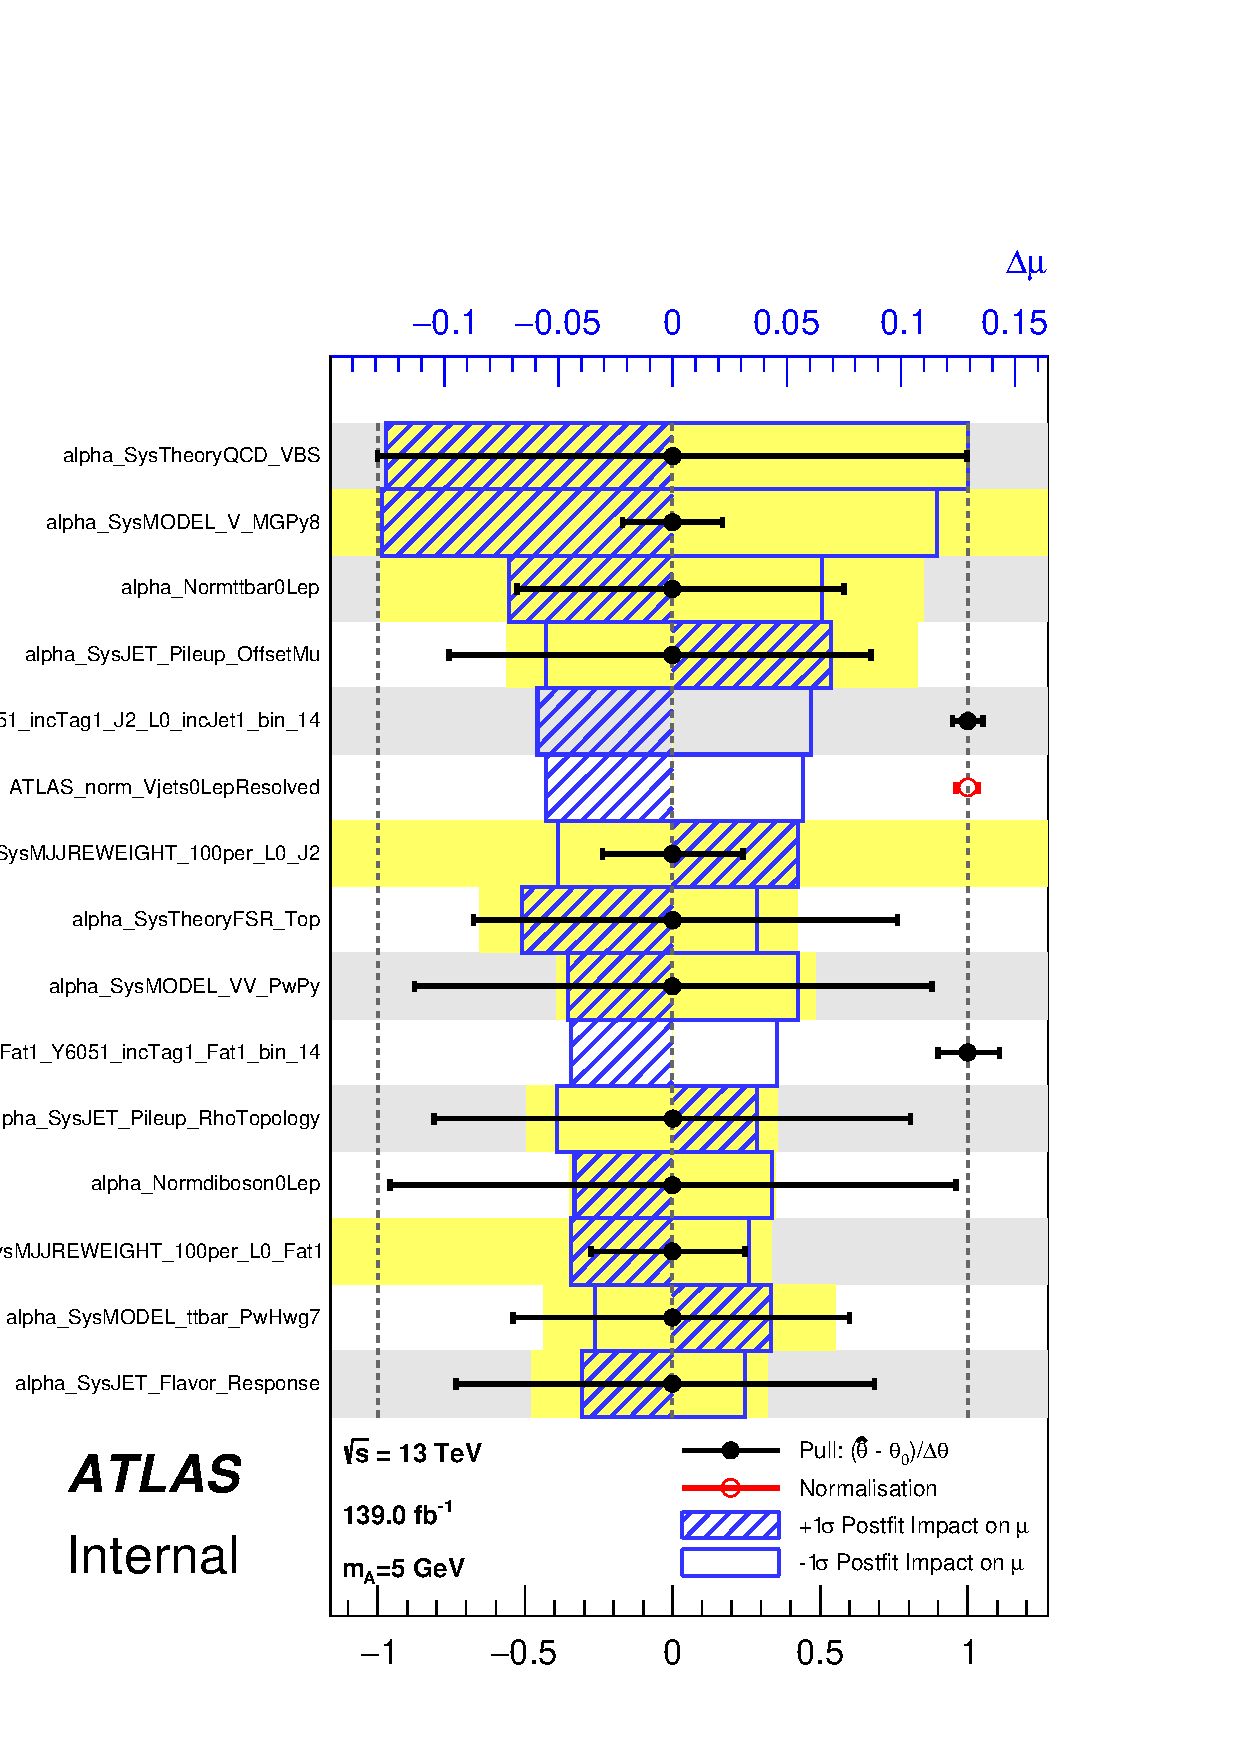
\includegraphics[width=0.5\textwidth]{figures/Fit_np_rank/pulls_mu_Asimov/pulls_mu_SemileptonicVBS_5.pdf}
        \caption{Ranking plot for unconditional fit ($\mu=1$) to asimov data in the full range, for the 1 lepton channel.}
       \label{fig:fit_1lep_ranking_all}
\end{figure}



%%%%%\clearpage
%%%%%\subsubsection{Left Bins Data Fit Results}
%%%%%
%%%%%According to the unblinding strategy, the fit model is inspected in the left side of our SRs using data fit; 
%%%%%the goal is to spot some problematics pulls that might appear in the final data fit.
%%%%%
%%%%%Figures \ref{fig:fit_1lep_fcc_left}-\ref{fig:fit_1lep_corr_left}
%%%%%show the pulls and the correlations respectively of the NPs used in the fit.
%%%%%
%%%%%\begin{figure}[ht]
%%%%%      \centering
%%%%%        \includegraphics[width=\linewidth]{figures/1lep/FitResults/left/NP_allExceptGammas.pdf}
%%%%%        \caption{Fit cross-check, unconditional fit ($\mu=1$) to data in the left bins only, for the 1 lepton channel only.}
%%%%%       \label{fig:fit_1lep_fcc_left}
%%%%%\end{figure}
%%%%%
%%%%%\begin{figure}[ht]
%%%%%      \centering
%%%%%        %\includegraphics[width=\linewidth]{figures/1lep/FitResults/left/corr_HighCorrNoMCStat.pdf}
%%%%%        \includegraphics[width=\linewidth]{figures/1lep/FitResults_SMApp/corr_HighCorrNoMCStat_Asimov.pdf}
%%%%%        \caption{Correlations for unconditional fit ($\mu=1$) to data in the left bins only, for the 1 lepton channel only.}
%%%%%       \label{fig:fit_1lep_corr_left}
%%%%%\end{figure}
%%%%%
%%%%%Similar constraints as found in the Asimov fit are found and confirmed in the left bins only fit. 
%%%%%They have been already discussed. 
%%%%%In addition, some pulls are found, they are:
%%%%%
%%%%%\begin{itemize}
%%%%%       \item \texttt{SysTheoryQCD\_W} has been found to be constrained in the asimov fit as well; 
%%%%%       a dedicated investigation has been done and the conclusion is reported in section \ref{sec:fit_1lep_QCDW}.
%%%%%
%%%%%       \item \texttt{SysTheoryISR\_ttbar} has been found to be constrained in the asimov fit as well; 
%%%%%       a dedicated investigation has been done and the conclusion is reported in section \ref{sec:fit_1lep_TheoryISR}.
%%%%%
%%%%%       \item \texttt{SysJET\_Flavor\_Response} it is the Flavor Response uncertainties for small-R jets, 
%%%%%       introduced in section \ref{subsec:bkg_uncer_qg}; 
%%%%%       the impact on the fitted $\mu$ is smaller than a few percent (Figure \ref{fig:fit:rankSingleStep0})
%%%%%       and 
%%%%%       it will be discussed and handled in the combined fit, in section~\ref{sec:fit_decorrStudies}.
%%%%%
%%%%%       \item \texttt{SysQG\_exp} this is the experimental uncertainty related to the track multiplicity of the small-R jets;
%%%%%       this is likely pulled due to modelling of the track multiplicity 
%%%%%       that are used as input of the final discriminant;
%%%%%       the impact on the fitted $\mu$ is smaller than a few percent (Figure \ref{fig:fit:rankSingleStep0})
%%%%%       and 
%%%%%       it will be discussed and handled in the combined fit, in section~\ref{sec:fit_decorrStudies}.
%%%%%
%%%%%\end{itemize}

~
